\documentclass[sigconf,review]{acmart}

\usepackage{tikz}
\usetikzlibrary{positioning,arrows.meta,fit,backgrounds,calc}
\definecolor{cData}{RGB}{219,234,254}\definecolor{cDataB}{RGB}{37,99,235}
\definecolor{cFeat}{RGB}{220,252,231}\definecolor{cFeatB}{RGB}{22,163,74}
\definecolor{cModel}{RGB}{255,237,213}\definecolor{cModelB}{RGB}{234,88,12}
\definecolor{cEval}{RGB}{237,233,254}\definecolor{cEvalB}{RGB}{124,58,237}

\setlength{\textfloatsep}{7pt plus 2pt minus 2pt}
\setlength{\floatsep}{5pt plus 2pt minus 2pt}
\setlength{\intextsep}{6pt plus 2pt minus 2pt}
\setlength{\abovecaptionskip}{4pt}
\setlength{\belowcaptionskip}{2pt}
\setlength{\abovedisplayskip}{5pt plus 2pt minus 2pt}
\setlength{\belowdisplayskip}{5pt plus 2pt minus 2pt}
\setlength{\abovedisplayshortskip}{3pt plus 2pt minus 2pt}
\setlength{\belowdisplayshortskip}{3pt plus 2pt minus 2pt}
\addtolength{\textheight}{18pt}

\AtBeginDocument{%
  \providecommand\BibTeX{{Bib\TeX}}}

\setcopyright{none}
\copyrightyear{2026}
\acmYear{2026}
\acmDOI{}
\acmConference[ICAIF '26]{ACM International Conference on AI in Finance}{2026}{}
\acmISBN{}

\begin{document}

\title{Learning Conditional TP2 Violation Opportunities in SPY American Call Options}
\subtitle{How Ensembling and the Decision Rule Reorder Model Comparisons}

\author{Pawel Polak}
\affiliation{%
  \institution{Stony Brook University}
  \city{Stony Brook}
  \state{New York}
  \country{USA}}
\email{pawel.polak@stonybrook.edu}

\author{Jyotir Manishkumar Patel}
\affiliation{%
  \institution{Stony Brook University}
  \city{Stony Brook}
  \state{New York}
  \country{USA}}
\email{jyotirmanishku.patel@stonybrook.edu}

\author{Omkar Lashkare}
\affiliation{%
  \institution{Stony Brook University}
  \city{Stony Brook}
  \state{New York}
  \country{USA}}
\email{omkarvilas.lashkare@stonybrook.edu}

\renewcommand{\shortauthors}{Polak, Patel, Lashkare}

\begin{abstract}
We study whether machine learning can identify economically meaningful total-positivity-inspired (TP2) violations in the SPY American call option surface. From conservative bid/ask TP2 episodes we construct strategy-level labels for the two structurally viable call strategies, T1 and K2, and evaluate on leakage-safe rolling train/validation/test splits over 2014--2026. The task is not to detect violations but to decide which episode-strategy pairs are worth trading: trading every one over 2021--2026 loses \$12.52M (Sharpe $-1.01$, 2 of 6 years profitable), yet three independent selectors -- LightGBM, an MLP, and a transformer attending to historical episodes over five domain-relevant distances -- each convert this into a positive portfolio under one fixed, causal rule (trade when calibrated probability $\ge 0.5$, no other tuning). This setting is our testbed for a methodological problem we argue is general and easy to miss: \textbf{comparing a single-seed model of one architecture against a multi-seed ensemble of another is uncontrolled, and correcting for it can reverse which model looks superior.} We show this concretely -- the MLP-versus-transformer ranking flips between single- and five-seed comparison, the same reversal recurs for an ALiBi-style attention extension, and selectivity curves confirm it is not a mere operating-point artifact -- with neither single-model gap separable at six test years (power $\approx0.26$). A capital-scaled backtest sharpens the caution: under realistic sizing both transformer variants fall far behind LightGBM and the MLP. Our contribution is not that any architecture wins, but a concrete demonstration of how, and why, such rankings mislead.
\end{abstract}

\begin{CCSXML}
<ccs2012>
 <concept>
  <concept_id>10010147.10010257.10010258.10010259</concept_id>
  <concept_desc>Computing methodologies~Machine learning</concept_desc>
  <concept_significance>500</concept_significance>
 </concept>
 <concept>
  <concept_id>10010405.10010481.10010485</concept_id>
  <concept_desc>Applied computing~Economics</concept_desc>
  <concept_significance>300</concept_significance>
 </concept>
</ccs2012>
\end{CCSXML}

\ccsdesc[500]{Computing methodologies~Machine learning}
\ccsdesc[300]{Applied computing~Economics}

\keywords{options, total positivity, machine learning, transformer, SPY, statistical arbitrage}

\maketitle

\section{Introduction}
\label{sec:intro}

No-arbitrage theory imposes shape restrictions on the option surface across strikes and maturities, and violations can indicate relative-value opportunities or market frictions. One such structure is total positivity of order two (TP2), which implies multiplicative inequalities between option prices arranged across strike and maturity. Prior work links TP2 violations to arbitrage strategies in theory, but detecting a violation is not the same as constructing a tradable, profitable one: bid/ask spreads, liquidity, stale quotes, early expiration, and regime changes can all turn a theoretical violation into a losing trade.

This paper studies TP2-inspired violations in SPY American call options -- highly liquid, with a dense surface across strikes and expirations. Although SPY options are American-style, a call's terminal payoff is still $\max(S_T-K,0)$, so expiration-payoff accounting is a clean way to study the economic content of TP2 violations, while still requiring care around execution, dividends, and early assignment of short calls.

Our central question is whether machine learning can distinguish profitable TP2 violation episodes from unprofitable ones using only information available at the violation date. We do not frame the task as violation detection; we first construct TP2 episodes and then ask whether a model should trade T1, trade K2, or skip. This framing matters because unconditional trading is not profitable: over 2021--2026, trading every valid T1/K2 episode under the \$1,000 convention loses \$12.52M in aggregate (Sharpe $-1.01$, only 2 of 6 years profitable). The research problem is therefore one of conditional selection, not detection.

We evaluate three independent selectors under rolling walk-forward splits -- each training on three years, calibrating on the following validation year, and testing once on the next -- so no test-year information enters training or calibration. Our baselines are a LightGBM classifier and an MLP on a common 48-feature dictionary. We then introduce a transformer that attends to historical TP2 episodes over five domain-relevant distances (time, option-surface location, short-leg structure, liquidity, lifecycle stage), and separately test augmenting this attention with a learned, ALiBi-style linear bias per distance; whether it beats plain attention depends on an ensembling choice (Section~\ref{sec:mvalibi-ablation}), so we adopt plain attention as primary.

A separate methodological contribution concerns trade selection: we replace an earlier validation-tuned threshold and a non-causal rank-based fraction rule (its cutoff depending on the full test period's predictions) with the simplest option -- trade whenever calibrated probability is at least 0.5, no tuning -- fixed a priori as the natural boundary for a calibrated probability (Section~\ref{sec:calibration}).

We also identify and correct a comparison bias easy to introduce unintentionally: naively comparing a single model fit for one architecture against a multi-seed ensemble for another favors whichever happens to have been ensembled, independent of which architecture is actually better. Correcting for it changes which model appears superior, and the underlying single-model gap is not statistically significant at six test years.

The contributions are fourfold: (1) a demonstration that model rankings in a trading pipeline turn on the \emph{interaction} between ensembling and the trade-selection rule, not architecture alone -- ensembling shifts both the model and its trade count, so seed-count-mismatched comparisons are uncontrolled; the effect recurs at three levels (MLP-versus-transformer, plain-versus-ALiBi attention, no-history ablation), survives a paired and a block bootstrap, and is separated from an operating-point artifact by selectivity curves; (2) a leakage-safe TP2 episode pipeline for SPY American calls with a causal trade-selection rule that recovers a substantial return from an otherwise unprofitable signal across three independent model families, the empirical setting for (1); (3) a capital-scaled backtest showing the transformer's edge over LightGBM/MLP shrinks sharply under realistic sizing (Sections~\ref{sec:addl-robustness}--\ref{sec:capitalscaled}); and (4) a TP2-specific historical-attention transformer and an MV-ALiBi extension, stress-tested for execution-cost/early-assignment and economic-exposure sensitivity (Section~\ref{sec:mvalibi-ablation}).

\section{Background and Related Work}
\label{sec:related}

\subsection{TP2 Inequalities and Options Arbitrage}
Total positivity of order 2 (TP2) is a shape restriction on call option prices arranged across strike and maturity: under the Black--Scholes model, and more generally a broad class of arbitrage-free pricing models, the ratio of a higher-strike to a lower-strike call price at the same maturity increases with time-to-expiry~\cite{glasserman2026tp2theory,glasserman2023convexity}. A TP2 violation is stronger than the absence of calendar-spread arbitrage and can indicate a relative-value opportunity empirically. Our episode-detection logic and normalized-exposure convention follow a companion study of TP2-violation trading on SPX options~\cite{glasserman2025tp2}, which finds violations rare, typically reverting quickly, and profitably tradable. The theoretical property itself~\cite{glasserman2026tp2theory} is proved for European-style, cash-settled index options; its proof conditions do not literally cover SPY, which is American-style on dividend-paying shares~\cite{cosma2020earlyexercise}. We do not claim the theorem extends to SPY -- we treat TP2 here as an empirically testable hypothesis about SPY prices, not an established property of them, and return to this gap explicitly in Section~\ref{sec:limitations}.

\subsection{Machine Learning for Options}
Machine learning applied to options has largely targeted implied-volatility surface fitting, delta-hedging, and derivative pricing; a separate line applies it directly to trading and market-making under realistic execution constraints~\cite{kearns2013mlmicrostructure}, and recent work predicts option returns cross-sectionally with machine learning on large panels~\cite{bali2023option}. We differ from all three: rather than forecasting a continuous quantity, we pose a binary trade/no-trade classification problem conditioned on an already-detected TP2 violation, evaluated purely on realized, cost-aware trading performance under rolling out-of-sample splits.

\subsection{Attention with Linear Biases}
Relative-position biases are a well-studied alternative to absolute positional embeddings in transformer attention, from learned relative-position representations~\cite{shaw2018self} and the T5 bucketed bias~\cite{raffel2020t5} to structural biases for graphs~\cite{ying2021graphormer} and functional long-context schemes~\cite{li2024fire}. ALiBi~\cite{press2022alibi} is the simplest such scheme: it replaces positional embeddings with a fixed linear penalty on attention logits, proportional to the distance between query and key positions, using a per-head slope fixed at initialization. This is effective for extrapolating to longer sequences in language modeling, where the relevant notion of distance is scalar token position. That notion of distance is not directly meaningful for TP2 episodes, which are better characterized by several simultaneous, domain-relevant distances rather than one. We test a multivariate generalization of ALiBi, described in Section~\ref{sec:transformer}, that replaces its single scalar distance and fixed slope with a five-dimensional distance vector and a slope learned, rather than fixed, separately per distance type and per attention head. This mechanism behaves exactly as designed at the level of what it learns, yet whether it improves trading performance depends on an ensembling choice, with neither direction statistically significant (Section~\ref{sec:mvalibi-ablation}); our primary transformer uses plain attention.

\section{Data and Episode Construction}
\label{sec:data}

\subsection{Data Source and Scope}
\label{sec:data-source}
We use SPY American call options from 2014--2026. The year 2013 is excluded: the data vendor reports 49{,}090 episodes in 2013 versus 438 in 2014, a discontinuity consistent with a vendor-side data-quality anomaly rather than a genuine change in market structure. After filtering to the T1/K2 strategy universe described below, our dataset contains 177{,}487 unique episodes, spanning 2014-02-03 to 2026-06-04. Table~\ref{tab:peryear} breaks these down by year: episode counts, candidate episode-strategy pairs (two per episode), and profitable-label base rate $\pi_t$.

\begin{table}[t]
\centering
\footnotesize
\begin{tabular}{rrrr@{\hskip 1.4em}rrrr}
\toprule
Yr & Epis. & Pairs & $\pi_t$ & Yr & Epis. & Pairs & $\pi_t$ \\
\midrule
2014 & 438 & 876 & 8.6\% & 2021 & 20{,}588 & 41{,}176 & 15.8\% \\
2015 & 140 & 280 & 1.1\% & 2022 & 6{,}604 & 13{,}208 & 16.0\% \\
2016 & 3{,}786 & 7{,}572 & 5.4\% & 2023 & 12{,}731 & 25{,}462 & 14.5\% \\
2017 & 12{,}284 & 24{,}568 & 45.8\% & 2024 & 34{,}167 & 68{,}334 & 15.9\% \\
2018 & 5{,}969 & 11{,}938 & 26.6\% & 2025 & 41{,}577 & 83{,}154 & 11.1\% \\
2019 & 4{,}151 & 8{,}302 & 41.6\% & 2026$^\dagger$ & 9{,}335 & 18{,}670 & 11.1\% \\
2020 & 25{,}717 & 51{,}434 & 72.5\% & & & & \\
\bottomrule
\end{tabular}
\caption{T1/K2 episodes, candidate pairs (two per episode), and profitable-label base rate $\pi_t$ by year. $\pi_t$ collapses from 45--73\% (2017--2020) to 11--16\% (2021--2026), the $\sim$4$\times$ label shift behind the calibration challenge (Section~\ref{sec:limitations}). 2013 excluded as a vendor anomaly (49{,}090 vs.\ 438 episodes in 2014). $^\dagger$2026 ends 2026-06-04 ($\approx$107 trading days).}
\label{tab:peryear}
\end{table}

\subsection{TP2 Episode Detection}
A TP2 episode begins when a conservative bid/ask option-price rectangle violates the TP2 inequality $C(K_1,T_1)\cdot C(K_2,T_2) < C(K_1^{\ast},T_2)\cdot C(K_2^{\ast},T_1)$ for strikes $K_1 < K_2$ and maturities $T_1 < T_2$, using rounded-up adjusted strikes $K_1^{\ast}, K_2^{\ast}$ where an exactly matching strike is unavailable. Unlike the companion SPX study~\cite{glasserman2025tp2} we do not additionally filter pairs against a vertical/calendar-spread no-arbitrage condition; that study reports such a filter removes under 2\% of violations with minimal profitability effect, so we expect little impact, but list it as a limitation (Section~\ref{sec:limitations}) rather than assuming it away.

\subsection{Episode Tracking}
\label{sec:episode-tracking}
The raw detector output is daily and rectangle-level: one economic TP2 violation can appear on many consecutive days, and treating each daily row as independent would inflate the sample and understate dependence across the splits of Section~\ref{sec:method}. We track episodes instead: consecutive appearances of the same strike/maturity pair are grouped into one pair episode, keyed on the pair's near-leg strike and maturity (the four-leg rectangle is a diagnostic, not part of the key, since rounding can shift it within an episode).

Over the full raw detection history, 2{,}430{,}220 daily violation rows collapse to 2{,}098{,}213 pair episodes. Episode duration is heavily right-skewed: 88.66\% of episodes are single-session events, the median duration is one session, and the maximum observed duration is 14 sessions. Of these raw pair episodes, 50.6\% end in true reversion (the TP2 inequality resolves) rather than expiring, losing a required leg, or failing a liquidity filter. This raw population is prior to the conservative bid/ask filter, the T1/K2 restriction, and the cost-aware labeling described below; the T1/K2 episode count used for modeling throughout the rest of this paper (177{,}487 episodes, Section~\ref{sec:data-source}) is a downstream, filtered subset of it.

We also build a lifecycle panel following every episode across a fixed event-time window (a 20-session pre-event lookback through expiration, indexed to the first violation day, event day 0). Figure~\ref{fig:lifecyclepath} plots the normalized TP2 pressure path: flat and slightly negative pre-event, spiking at day 0 by construction, then decaying toward zero -- making the reversion and duration statistics above auditable rather than only asserted. Although the panel runs through expiration, every lifecycle feature used as model input is truncated at event day 0 (the ``$\le0$'' construction) -- only pre- and at-signal pressure, observability, and liquidity summaries enter $F^{\ast}$, never post-signal rows.

\begin{figure}[t]
\centering
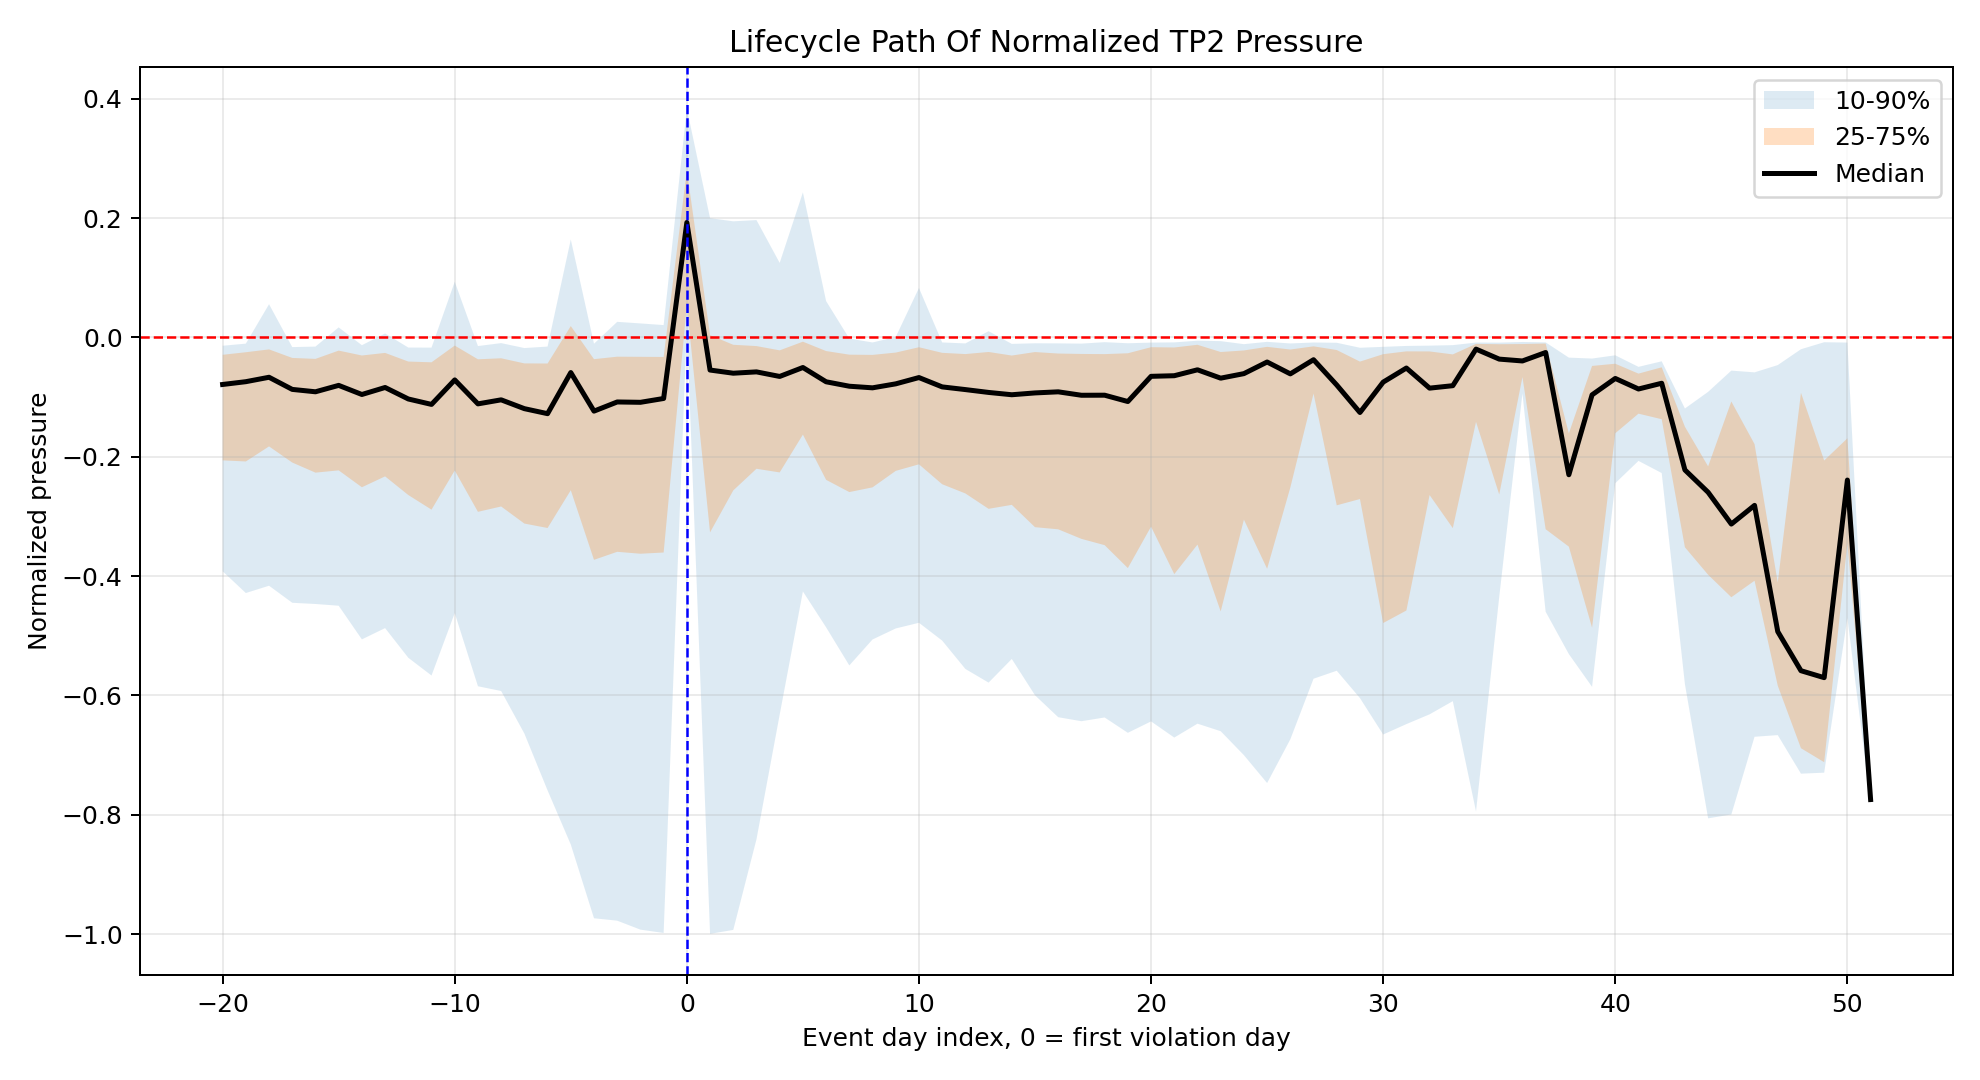
\includegraphics[width=0.66\linewidth]{figures/lifecycle_normalized_pressure_band.png}
\caption{Lifecycle path of normalized TP2 pressure -- $(C(K_1^{\ast},T_2)C(K_2^{\ast},T_1) - C(K_1,T_1)C(K_2,T_2))$ divided by the sum of both sides -- from 20 sessions before a violation's first appearance through expiration, for every conservative bid/ask episode in the 2014--2026 sample. Dashed line: event day 0 (first violation, pressure spikes by construction); solid line: median; bands: 10--90 and 25--75 percentile range.}
\label{fig:lifecyclepath}
\end{figure}

\subsection{Label Construction and Transaction Costs}
\label{sec:labels}
The primary label policy holds positions to expiration and uses the terminal intrinsic payoff for the selected leg. Hold-to-expiry is the natural primary policy here because 88.66\% of episodes are single-session (Section~\ref{sec:episode-tracking}), so most never present a distinct post-signal reversion exit; on the small subset of selected episodes that do carry a defined true-reversion exit, closing at reversion instead of expiry does not improve on hold-to-expiry, so we retain the simpler policy. Our realized-return calculation is cost-aware rather than a naive mid-price backtest: the entry leg of every trade is executed at the full bid-ask spread (long positions buy at the ask, short positions sell at the bid), and a commission of \$0.65 per contract is charged per leg, matching Interactive Brokers' published IBKR Lite fixed-rate US options commission.\footnote{\url{https://www.interactivebrokers.com/en/pricing/commissions-options.php}, accessed 2026.} Realized return is normalized by the trade's own gross exposure and expressed in dollar terms via a \$1{,}000 fixed-exposure convention, so P\&L is directly interpretable as a percentage return regardless of the option's actual price level -- necessary here since raw, un-normalized exposures range from a median of \$7--\$11 to a maximum of \$814{,}000 per trade.

\subsection{Strategy Restriction: T1 and K2}
We restrict to the T1 and K2 strategy denominations, both of which short the shorter-dated leg of the TP2 violation -- a structural prior decided on theoretical grounds before any model training, since the excluded T2 and K1 both short the longer-dated leg, exposing the position to a longer horizon for an adverse move to develop. We test this prior empirically: Section~\ref{sec:lgbm-scope} trains an unrestricted four-strategy classifier and shows T2/K1 lose heavily, consistent with the structural argument.

\section{Methodology}
\label{sec:method}

Figure~\ref{fig:pipeline} details the full pipeline described in this section, from raw SPY option quotes through the shared calibration and selection stage that produces the evaluated portfolio in Section~\ref{sec:results}.

\begin{figure*}[t]
\centering
\resizebox{0.82\textwidth}{!}{%
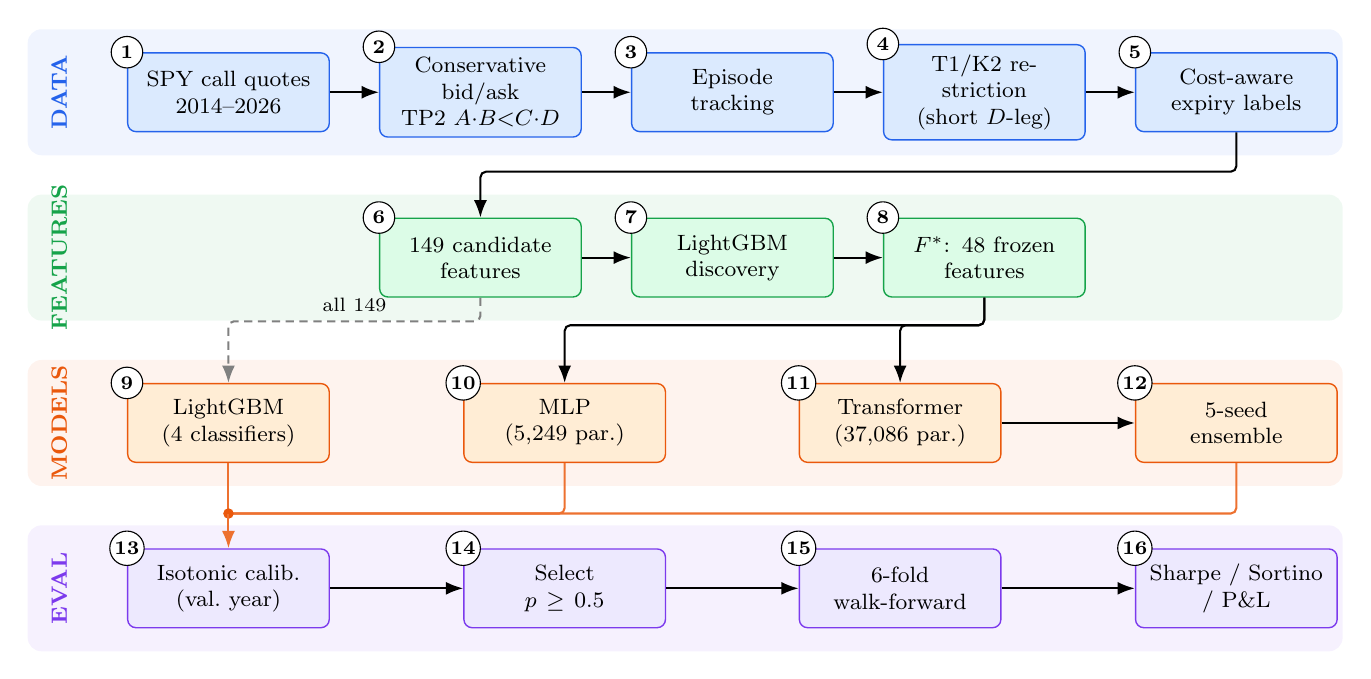
\begin{tikzpicture}[
  every node/.style={font=\footnotesize},
  b/.style={draw, rounded corners=3pt, align=center, text width=2.3cm, minimum height=1.0cm, inner sep=1.3mm, line width=0.5pt},
  bd/.style={b, fill=cData, draw=cDataB}, bf/.style={b, fill=cFeat, draw=cFeatB},
  bm/.style={b, fill=cModel, draw=cModelB}, be/.style={b, fill=cEval, draw=cEvalB},
  arr/.style={-{Latex[length=2.2mm]}, line width=0.75pt, rounded corners=2pt},
  mrg/.style={line width=0.75pt, rounded corners=2pt, cModelB!85},
  brc/.style={-{Latex[length=2.2mm]}, line width=0.75pt, densely dashed, gray, rounded corners=2pt},
  sn/.style={circle, draw, fill=white, font=\scriptsize\bfseries, inner sep=0.3mm, minimum size=4mm}
]
\def\ry{0}\def\rf{-2.1}\def\rm{-4.2}\def\re{-6.3}
\begin{scope}[on background layer]
  \fill[cDataB!7,  rounded corners=5pt] (-2.55,0.80)  rectangle (14.15,-0.80);
  \fill[cFeatB!7,  rounded corners=5pt] (-2.55,-1.30) rectangle (14.15,-2.90);
  \fill[cModelB!7, rounded corners=5pt] (-2.55,-3.40) rectangle (14.15,-5.00);
  \fill[cEvalB!7,  rounded corners=5pt] (-2.55,-5.50) rectangle (14.15,-7.10);
\end{scope}
\node[bd] (n1) at (0,\ry)    {SPY call quotes\\2014--2026};
\node[bd] (n2) at (3.2,\ry)  {Conservative bid/ask\\TP2 $A{\cdot}B{<}C{\cdot}D$};
\node[bd] (n3) at (6.4,\ry)  {Episode\\tracking};
\node[bd] (n4) at (9.6,\ry)  {T1/K2 restriction\\(short $D$-leg)};
\node[bd] (n5) at (12.8,\ry) {Cost-aware\\expiry labels};
\node[bf] (n6) at (3.2,\rf) {149 candidate\\features};
\node[bf] (n7) at (6.4,\rf) {LightGBM\\discovery};
\node[bf] (n8) at (9.6,\rf) {$F^{\ast}$: 48 frozen\\features};
\node[bm] (n9)  at (0,\rm)    {LightGBM\\(4 classifiers)};
\node[bm] (n10) at (4.27,\rm) {MLP\\(5{,}249 par.)};
\node[bm] (n11) at (8.53,\rm) {Transformer\\(37{,}086 par.)};
\node[bm] (n12) at (12.8,\rm) {5-seed\\ensemble};
\node[be] (n13) at (0,\re)    {Isotonic calib.\\(val.\ year)};
\node[be] (n14) at (4.27,\re) {Select\\$p\!\ge\!0.5$};
\node[be] (n15) at (8.53,\re) {6-fold\\walk-forward};
\node[be] (n16) at (12.8,\re) {Sharpe / Sortino\\/ P\&L};
\draw[arr] (n1)--(n2); \draw[arr] (n2)--(n3); \draw[arr] (n3)--(n4); \draw[arr] (n4)--(n5);
\draw[arr] (n5.south) -- ++(0,-0.5) -| (n6.north);
\draw[arr] (n6)--(n7); \draw[arr] (n7)--(n8);
\draw[arr] (n8.south) -- ++(0,-0.35) -| (n11.north);
\draw[arr] (n8.south) -- ++(0,-0.35) -| (n10.north);
\draw[brc] (n6.south) -- ++(0,-0.3) -| (n9.north) node[pos=0.25,above,black,font=\scriptsize]{all 149};
\draw[arr] (n11)--(n12);
\coordinate (jn) at (0,-5.35);
\draw[mrg] (n10.south) |- (jn);
\draw[mrg] (n12.south) |- (jn);
\draw[mrg] (n9.south) -- (jn);
\fill[cModelB] (jn) circle (1.9pt);
\draw[arr, cModelB!85] (jn) -- (n13.north);
\draw[arr] (n13)--(n14); \draw[arr] (n14)--(n15); \draw[arr] (n15)--(n16);
\foreach \n/\l in {n1/1,n2/2,n3/3,n4/4,n5/5,n6/6,n7/7,n8/8,n9/9,n10/10,n11/11,n12/12,n13/13,n14/14,n15/15,n16/16}
  \node[sn] at (\n.north west) {\l};
\node[rotate=90, cDataB,  font=\bfseries\footnotesize] at (-2.15,\ry) {DATA};
\node[rotate=90, cFeatB,  font=\bfseries\footnotesize] at (-2.15,\rf) {FEATURES};
\node[rotate=90, cModelB, font=\bfseries\footnotesize] at (-2.15,\rm) {MODELS};
\node[rotate=90, cEvalB,  font=\bfseries\footnotesize] at (-2.15,\re) {EVAL};
\end{tikzpicture}
}
\caption{End-to-end pipeline, numbered 1--16. Steps 1--5 build the episode-level dataset; Step 6 exposes 149 candidate features; Steps 7--8 select the frozen 48-feature $F^{\ast}$ dictionary, while LightGBM (Step 9) trains on all 149 independently of $F^{\ast}$ (dashed). Steps 10--12 train the MLP, transformer, and its 5-seed ensemble from $F^{\ast}$. The three independent scorers (Steps 9, 10, 12) converge on one identical shared downstream -- calibration, $p\ge0.5$ selection, 6-fold evaluation, and metrics (Steps 13--16).}
\label{fig:pipeline}
\end{figure*}

\subsection{Rolling Evaluation Protocol}
We use a six-fold rolling walk-forward scheme: a three-year training window, a one-year validation year, and a one-year test year, rolling forward one year at a time to cover test years 2021--2026 (Table~\ref{tab:folds}). No test-year information enters training, calibration, or feature scaling for that fold: the scaler is fit on training years only, and calibration (Section~\ref{sec:calibration}) on the validation year only. Section~\ref{sec:window} separately tests an expanding-window alternative.

\begin{table}[H]
\centering
\footnotesize
\begin{tabular}{lll}
\toprule
Train years & Validation year & Test year \\
\midrule
2017--2019 & 2020 & 2021 \\
2018--2020 & 2021 & 2022 \\
2019--2021 & 2022 & 2023 \\
2020--2022 & 2023 & 2024 \\
2021--2023 & 2024 & 2025 \\
2022--2024 & 2025 & 2026 \\
\bottomrule
\end{tabular}
\caption{The six rolling walk-forward folds used for every model and result in this paper: train on `Train years', calibrate (isotonic) on `Validation year', evaluate once, with no further tuning, on `Test year'. No test year appears in that fold's training or validation data.}
\label{tab:folds}
\end{table}

\subsection{Feature Selection}
We use LightGBM~\cite{ke2017lightgbm} as a feature-discovery tool, separate from its role as a trading model (Section~\ref{sec:lgbm-scope}). From 149 candidate features spanning eight semantic blocks (market, short-leg structure, option risk, surface location, liquidity, TP2 geometry, strategy/calendar, lifecycle pressure), we select 48 features $F^{\ast}$, dominated by the market and short-leg-structure groups (12 and 10 features), using a composite score combining gain-based importance, permutation importance, and a temporal-stability penalty across folds. $F^{\ast}$ is selected once and frozen: importance is pooled over all six folds (train years 2017--2024, validation years 2020--2025) and stability is the fraction of the twelve fold$\times$strategy runs placing a feature in the top 30. Because this single set is reused across folds, its selection touches validation years (2020--2025) that overlap later test years -- a feature-selection leakage not removed by the per-fold split of Section~\ref{sec:method}, which we leave to future work to close by re-selecting within each fold. Only the selected feature values feed the MLP and transformer -- LightGBM's predictions, leaf indices, and importance scores are never used downstream -- so Section~\ref{sec:results} compares three independent approaches on a shared, inspectable feature set rather than a stacked ensemble.

\noindent\textbf{Implementation (all models).} Every model uses the six rolling folds, standardizes features on training data, fits isotonic calibration on the validation year, and selects at $p\ge0.5$; single-seed rows use the fixed default seed 42 (set a priori, not the best of several) and 5-seed ensembles average seeds \{42,101,202,303,404\} before one calibration. LightGBM: 350 trees, lr 0.04, 31 leaves, min-child 30, subsample/colsample 0.8, balanced class weights. MLP (5{,}249 params): Adam, lr $10^{-3}$, $L_2$ $10^{-4}$, batch 1024, $\le$80 epochs, early-stop patience 8. Transformer (37{,}086 params): hidden 64, 4 heads, 5 distances, $\le$64 history, AdamW lr $3{\times}10^{-5}$, weight decay $10^{-4}$, 8\% warm-up, grad-clip 1.0, $\le$25 epochs, val-loss checkpoint, plus a Huber return-auxiliary loss.

\subsection{LightGBM Model}
\label{sec:lgbm-scope}
Our LightGBM model trains four independent binary classifiers, one per strategy denomination (T1, T2, K1, K2), on the full 149-candidate feature set and all four denominations -- letting us test the T1/K2 structural prior directly. Its T1/K2 sub-models evaluate on an episode population identical to the MLP and transformer (177{,}487 episodes each, zero difference in episode-ID sets, matching base profitability rates of 25.33\%/23.67\%), so Section~\ref{sec:results}'s comparison is not confounded by a different data population.

\subsection{MLP Baseline}
The MLP baseline is a feedforward network with layer sizes 48, 64, 32, and 1 (ReLU activations, 5{,}249 parameters total), trained on the selected feature dictionary $F^{\ast}$. This model tests whether the selected features alone, without any sequence or historical-attention modeling, contain tradable signal.

\subsection{TP2 Historical-Attention Transformer}
\label{sec:transformer}
Each candidate episode-strategy pair is encoded as a token combining its $F^{\ast}$ feature values, a strategy embedding, and calendar features. The current token attends to up to 64 prior episode tokens, drawn only from strictly earlier calendar days -- the 64 most recently-dated tokens before the current episode's day, in chronological order and zero-padded/masked when fewer exist, selected by date alone and never by any label or outcome (so the window is causal and reproducible) -- via a single cross-attention block with four heads and hidden dimension 64 (37{,}086 parameters total, roughly seven times the size of the MLP baseline). The attention logit for head $h$ between the current token $i$ and a historical token $j$ is
\[
a_{ij}^{h} \;=\; \frac{q_i \cdot k_j}{\sqrt{d}} \;+\; \text{(same/cross-strategy bonus)},
\]
i.e.\ plain scaled dot-product cross-attention with a same/cross-strategy bonus added (no distance-based penalty; Section~\ref{sec:mvalibi-ablation} tests a distance-biased variant we did not adopt). Trained with binary cross-entropy on the profitability label plus an auxiliary Huber-loss term on realized return, using AdamW (learning rate $3\times10^{-5}$, linear warm-up over the first 8\% of training, gradient clip 1.0, weight decay $10^{-4}$). The model checkpoints on lowest validation loss rather than best validation ranking metric; an earlier iteration checkpointed on the ranking metric, which let epochs with degrading calibration survive whenever ranking still looked acceptable.

\subsection{MV-ALiBi Distance-Bias Ablation: An Ensembling-Sensitive Result}
\label{sec:mvalibi-ablation}
Section~\ref{sec:related} motivates a natural extension: bias each attention logit by a learned function of several domain-relevant distances between episodes, generalizing ALiBi's single scalar distance penalty~\cite{press2022alibi}. We built and tested exactly this extension before deciding whether to adopt it, rather than including it in the architecture description above by default. The extended attention logit is
\[
a_{ij}^{h} \;=\; \frac{q_i \cdot k_j}{\sqrt{d}} \;-\; m_h^{\top} d_{ij} \;+\; \text{(same/cross-strategy bonus)},
\]
where $d_{ij}$ is a five-dimensional vector of distances between episode $i$ and historical episode $j$ -- time elapsed, option-surface location, short-leg structure, liquidity, and lifecycle stage -- and $m_h$ is a learned, strictly positive per-head slope vector obtained via a softplus transform, added as 20 extra parameters (5 distances $\times$ 4 heads) on top of the 37{,}086-parameter base architecture.

The mechanism behaves as designed: despite the five distance types spanning very different raw scales, the learned slopes converge to a tight 0.26--0.27 band across all types, heads, and (across 30 models) initializations, compensating for the differing units rather than being dominated by the largest-magnitude distance.

Whether the distance-bias term helps depends on an ensembling choice, exactly as for the MLP-versus-transformer comparison (Section~\ref{sec:seedcount}). At matched single seed, plain attention wins (Sharpe 1.73 vs.\ 1.51, with higher P\&L, Sortino, and smaller drawdown); at matched 5-seed ensemble the ranking reverses (distance-biased 2.36 vs.\ plain 2.18; Table~\ref{tab:alibi-ablation}). Neither reaches significance: two-sided sign tests give $p=0.219$ (single, plain wins 5/6) and $p=1.000$ (5-seed, a 3--3 split), both with mean-difference CIs including zero, and a block bootstrap~\cite{kunsch1989} agrees (single-seed CI $[-\$162.3\text{K}, \$405.4\text{K}]$; five-seed $[-\$134.9\text{K}, \$110.4\text{K}]$) -- both underpowered at $n=6$. We report both comparisons rather than the favorable one, and adopt plain attention as primary for the single-seed result and architectural simplicity (20 fewer parameters), while stating plainly that the 5-seed evidence favors the distance-biased variant instead.

\begin{table}[t]
\centering
\footnotesize
\resizebox{\linewidth}{!}{%
\begin{tabular}{llrrrr}
\toprule
Model & Seeds & Total P\&L & Sharpe & Sortino & Max DD \\
\midrule
Transformer (plain attention) & 1 & \$686K & 1.73 & 1.70 & $-$\$242K \\
Transformer (+ MV-ALiBi distance bias) & 1 & \$570K & 1.51 & 1.24 & $-$\$268K \\
Transformer (plain attention) & 5 & \$695K & 2.18 & 2.98 & $-$\$128K \\
Transformer (+ MV-ALiBi distance bias) & 5 & \$704K & 2.36 & 3.72 & $-$\$91K \\
\bottomrule
\end{tabular}%
}
\caption{Matched seed-count comparison, identical protocol otherwise (same features, folds, val-loss checkpointing, calibration, and $p\ge0.5$ selection rule): plain attention wins at single-seed, the distance-biased variant wins at 5-seed ensemble, and neither difference is statistically significant (main text).}
\label{tab:alibi-ablation}
\end{table}

\subsection{How Much Does Historical Attention Add? No-History and Permuted-History Ablations}
\label{sec:nohistory}
Sections~\ref{sec:seedcount} and~\ref{sec:mvalibi-ablation} compare architectures that all retain historical cross-attention; neither isolates whether attending to history -- rather than just the shared 48-feature dictionary -- is what makes the transformer competitive. We run two controls, both otherwise identical (features, folds, val-loss checkpointing, calibration, $p\ge0.5$). The \emph{no-history} variant removes cross-attention entirely (the input projection feeds the classification head directly; 16{,}130 parameters). Its apparent effect depends sharply on ensembling, exactly as Section~\ref{sec:seedcount} warns: at matched single seed (42) removing history looks decisive (Sharpe 1.73$\to$0.87, positive years 6/6$\to$4/6), but at matched five-seed ensemble the gap shrinks to Sharpe 1.81 (\$719.9K, 6/6) versus the full model's 2.18 -- a real but modest $\approx0.37$ gain, not a near-halving. The \emph{permuted-history} variant is more revealing: it keeps the full attention architecture and all 37{,}086 parameters but attends to 64 \emph{randomly chosen} strictly-earlier episodes instead of the 64 most-recent ones. At five seeds it reaches Sharpe 2.14 (\$652.4K, 6/6) -- almost the full model's 2.18. So the gain over no-history comes from the attention pathway itself, not the relevance of the attended episodes: swapping the most-recent history for random earlier history costs only $\approx0.04$ Sharpe. We therefore report historical attention as a modest, seed-count-sensitive contributor whose benefit is largely mechanism, not specific content -- and the single-seed ablation as a further caution against reading one seed as an architectural verdict.

\subsection{Probability Calibration and Trade Selection}
\label{sec:calibration}
For every model, we fit isotonic regression calibration~\cite{zadrozny2002transforming} on validation-year predictions and labels only, never on test-year labels, and apply the fitted map unchanged to the test year. For multi-seed ensembles, raw probabilities are averaged across seeds before a single calibration is fit. The choice of calibrator family is not load-bearing: refitting per fold as Platt scaling instead of isotonic selects a near-identical trade set (within 0.3\% on $N$) with essentially equal test calibration (ECE 0.075 vs.\ 0.072). The selected count itself carries real sampling uncertainty, however -- a block bootstrap over trading dates gives a 95\% CI of roughly $\pm25$--$30\%$ on $N$ (e.g., the five-seed transformer's 14{,}338 trades, CI $[10.3\text{K}, 19.0\text{K}]$).

The trade-selection rule has no tunable parameters: select any episode-strategy pair whose calibrated probability is at least 0.5, else skip -- causal by construction, since it depends only on the current trade's own probability. This is the natural boundary for a calibrated binary probability ($p\ge0.5$ means more likely profitable than not), fixed a priori and identical across every model and fold. We rejected two alternatives during development: a validation-tuned absolute threshold, prone to degenerate cutoffs that chase rare winners; and a rank-based top-$K$ fraction, non-causal because its cutoff is a quantile of the whole test period's predictions. As a diagnostic only, both the early (2021--2023) and late (2024--2026) halves are solidly profitable under the unmodified rule (Sharpe 1.17 and 2.88), so its behavior is not concentrated in one stretch.

\section{Results}
\label{sec:results}

All results in this section use the identical evaluation protocol described in Section~\ref{sec:method}: isotonic calibration fit on the validation year only, the $p \ge 0.5$ selection rule, and daily-grouped Sharpe ratio, Sortino ratio, and maximum drawdown computed from the same code path for every model. We annualize the daily-grouped Sharpe as $\sqrt{252}\,\bar{r}_d/\sigma(r_d)$, where $r_d$ is a model's total normalized P\&L on trading day $d$ over its selected trades; days with no selected trade are omitted, so this statistic rises with a model's trade density and is not directly comparable across models that differ substantially in trade count $N$ (Table~\ref{tab:consolidated}).

\subsection{Unconditional Baseline}
Trading every T1/K2 episode with no model at all, over the six 2021--2026 test years, loses \$12.52M in aggregate across 250{,}004 candidate episode-strategy pairs -- the 177{,}487 episodes each contribute one T1 and one K2 candidate (Sharpe $-1.01$, Sortino $-2.12$, maximum drawdown $-\$24.51$M, win rate 12.9\%, 2 of 6 years profitable). This is the floor every learned model must clear.

\subsection{Consolidated Model Comparison}
\label{sec:seedcount}
Table~\ref{tab:consolidated} reports every model, at every seed count we evaluated, alongside the unconditional baseline, under the identical selection rule and metrics. LightGBM, the MLP, and the transformer all convert the unconditional loss into a substantial positive return. Two reference baselines (last two rows) bracket the result: an L2-regularized logistic regression on the same $F^{\ast}$ features -- a purely linear selector with no hidden layer -- already recovers \$2.02M (Sharpe 2.27), close to the neural models and above LightGBM, indicating that most of the tradable signal is linear in the selected features rather than architecture-specific -- consistent with evidence that tree and linear models remain strong on tabular data~\cite{grinsztajn2022why,shwartzziv2022tabular,gorishniy2021revisiting}; while random selection at matched trade count ($N{=}14{,}258$, mean of 30 draws) loses \$0.77M (Sharpe $-1.14$), confirming the learned gains are not a mechanical consequence of how many trades are taken.

\begin{table}[t]
\centering
\footnotesize
\resizebox{\linewidth}{!}{%
\begin{tabular}{llrrrrrrrr}
\toprule
Method & Seeds & Trades & Total P\&L & Sharpe & Sortino & Win\% & $\bar r$\% & Skew & Pos.\ yrs \\
\midrule
Unconditional & -- & 250{,}004 & $-$\$12.52M & $-$1.01 & $-$2.12 & 12.9 & $-$5.0 & 16.6 & 2/6 \\
LightGBM & 1 & 19{,}636 & \$682K & 1.25 & 1.12 & 50.6 & 3.5 & 9.4 & 5/6 \\
MLP & 1 & 14{,}258 & \$1.41M & 2.60 & 6.89 & 54.0 & 9.9 & 9.6 & 6/6 \\
MLP & 5 & 24{,}977 & \$3.43M & 1.66 & 6.12 & 33.0 & 13.7 & 8.9 & 4/6 \\
Transformer (plain) & 1 & 16{,}435 & \$686K & 1.73 & 1.70 & 57.9 & 4.2 & 1.1 & 6/6 \\
Transformer (plain) & 5 & 14{,}338 & \$695K & 2.18 & 2.98 & 60.0 & 4.8 & 1.8 & 6/6 \\
Transformer (ALiBi) & 1 & 15{,}015 & \$570K & 1.51 & 1.24 & 61.0 & 3.8 & $-$2.3 & 6/6 \\
Transformer (ALiBi) & 5 & 14{,}648 & \$704K & 2.36 & 3.72 & 60.1 & 4.8 & 1.0 & 6/6 \\
\midrule
Logistic (L2) & 1 & 13{,}841 & \$2.02M & 2.27 & 4.20 & 53.5 & 14.6 & 5.5 & 5/6 \\
Random @$N$ & -- & 14{,}258 & $-$\$0.77M & $-$1.14 & -- & -- & -- & -- & -- \\
\bottomrule
\end{tabular}%
}
\caption{Every model and seed count evaluated -- the transformer as both plain attention and the MV-ALiBi variant (Section~\ref{sec:mvalibi-ablation}) -- plus the unconditional, a linear (L2-logistic), and a random-at-matched-$N$ baseline, over all six 2021--2026 test years (Table~\ref{tab:folds}). `Seeds': independently trained models whose raw probabilities are averaged before one calibration step. `Trades': episode-strategy pairs traded ($p\ge0.5$ for a learned model, Section~\ref{sec:calibration}). $\bar r$\%: mean per-trade normalized return; Skew: skewness of per-trade returns. Dollar figures under the \$1{,}000-per-trade convention; Sharpe/Sortino annualized on daily-grouped returns; `Pos.\ yrs' counts positive-P\&L years. The two most profitable rows (MLP-5, Logistic) also carry the highest right-skew and lowest win rate -- large-P\&L totals concentrated in a few outsized winners, which Sharpe penalizes and Sortino rewards.}
\label{tab:consolidated}
\end{table}

Comparing a single MLP fit against a five-seed transformer ensemble alone would not be controlled: it favors whichever model happened to be ensembled. Table~\ref{tab:consolidated} reports both architectures at matched seed counts (1 and 5), same ensembling procedure for both. Ensembling moves the two architectures in opposite directions: it improves the transformer's Sharpe (1.73$\to$2.18) and drawdown ($-$\$242K$\to-$\$128K), but degrades MLP's consistency (six of six $\to$ four of six profitable years) even as total P\&L triples -- win rate falls from 54.0\% to 33.0\% as averaging pulls predictions toward the mean and, after recalibration, lets more lower-quality trades cross the threshold.

Seed dispersion sharpens the point. Across the same five seeds, the single-seed MLP's test Sharpe ranges 1.47--2.60 (median 2.07, interquartile mean 2.07) -- the 2.60 in Table~\ref{tab:consolidated} is the fixed default seed 42, the most favorable of the five, so a single-seed MLP estimate varies by more than the nominal single-versus-ensemble gap. The plain transformer is far tighter (single-seed Sharpe 1.50--1.81, median 1.73, IQM 1.73), and its five-seed ensemble (2.18) exceeds \emph{every} single seed -- so ensembling helps the transformer consistently while the MLP's point estimate is simply too noisy to rank architectures on. All single-seed rows use the same fixed seed 42, set a priori, not the best of several.

Once controlled for ensembling, the ranking does not hold cleanly either way: single MLP beats single transformer on Sharpe, but the five-seed ensembles reverse this on Sharpe, Sortino, and drawdown. A paired bootstrap~\cite{efron1993bootstrap} (20{,}000 resamples) and a sign test (reported two-sided) on year-by-year P\&L differences find neither seed count significant: single-seed $p=0.688$ (4 of 6 years favor MLP), five-seed $p=1.000$ (an even 3--3 split). The five-seed paired-bootstrap CI $[\$18.5\text{K}, \$927.1\text{K}]$ excludes zero only because MLP's winning years are far larger (up to \$1.33M in 2021) than the transformer's (at most \$136K in 2026). With just six paired years the sign test's power is only $\approx0.26$ against a model that truly wins 80\% of years, so we read these nulls as underpowered, not as evidence the architectures are equivalent -- the same benchmarking-variance caution raised across machine learning~\cite{bouthillier2021accounting,dodge2019show,agarwal2021deep,melis2018state,lucic2018gans} and, for backtests specifically, in the data-snooping literature~\cite{white2000reality,hansen2005spa,harvey2016crosssection}. These two tests disagree at five-seed specifically; we report both rather than the more favorable one. A trade-dependence-aware block bootstrap~\cite{kunsch1989} (Section~\ref{sec:addl-robustness}) agrees: neither seed count reaches significance (single-seed CI $[-\$676.5\text{K}, \$2.53\text{M}]$; five-seed CI $[-\$2.16\text{M}, \$10.18\text{M}]$, both including zero).

We also verified the T1/K2 restriction empirically: LightGBM trained on all four denominations loses \$37.23M unrestricted (Sharpe $-1.76$, 1/6 profitable years), confirming T2/K1 are structurally unprofitable, not merely theoretically disfavored.

\subsection{Selectivity Curves: Is the Ranking an Operating-Point Artifact?}
\label{sec:selectivity}
Because ensembling changes not only the models but also how many trades each takes ($N$ moves $+75\%$ for the MLP but $-13\%$ for the transformer), the compared MLP and plain-transformer cells of Table~\ref{tab:consolidated} sit at different operating points -- so a raw Sharpe comparison could reflect selectivity rather than model quality. Figure~\ref{fig:selectivity} controls for this directly: sweeping the calibrated threshold traces each model's Sharpe and Sortino as a function of $N$. Two things are clear at \emph{matched} $N$. First, the single-seed MLP dominates both transformer variants across the entire range (Sharpe $\approx2.2$--$2.6$ versus $1.0$--$1.7$ for the single transformer and $1.9$--$2.3$ for the five-seed transformer at $N\approx10$--$16$K), so the MLP's advantage is not an operating-point artifact. Second, within the transformer family the five-seed ensemble sits above the single seed at every $N$ -- ensembling genuinely helps the transformer, independent of the trade-count shift. The confound the curves rule out is thus \emph{cross-architecture} seed-count mismatch, not the within-transformer ensembling effect.

\begin{figure}[t]
\centering
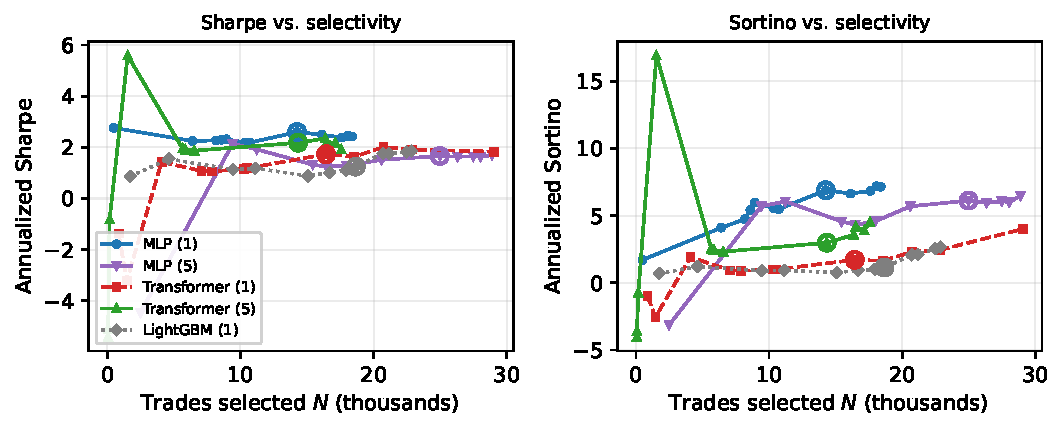
\includegraphics[width=\linewidth]{figures/selectivity_curves.pdf}
\caption{Selectivity curves: annualized Sharpe (left) and Sortino (right) versus number of trades $N$ as the calibrated selection threshold sweeps $0.30$--$0.85$. Open circles mark each model's $p\ge0.5$ operating point (the rows of Table~\ref{tab:consolidated}). At matched $N$ the single-seed MLP leads throughout, and the five-seed transformer leads the single-seed transformer throughout.}
\label{fig:selectivity}
\end{figure}

\subsection{T1/K2 Strategy-Level Breakdown}
\label{sec:t1k2breakdown}
Splitting each model at a matched single seed (42) by denomination -- without mixing single-seed baselines against a five-seed transformer, as an earlier version did -- shows K2 as the common source of conditional profitability. For the single-seed MLP, K2 supplies \$1.21M of \$1.41M (Sharpe 2.66 versus 1.62 for T1); the single-seed transformer is starker, its entire net gain being K2 (\$717K, Sharpe 2.60) against a small T1 loss ($-$\$31K) that turns positive (\$274K) only once ensembled -- another instance of ensembling changing the picture. LightGBM is the most balanced of the three, so the result is not confined to a single model or denomination.

\subsection{Annual Out-of-Sample Performance}
Each selected trade is sized to a fixed \$1{,}000 normalized exposure regardless of outcome, with no reinvestment, so we report per-year totals rather than a compounding return series. Figure~\ref{fig:annualpnl} plots test-year P\&L by model and year for the unconditional baseline and the three learned models at a matched single seed (LightGBM, MLP, transformer). Unconditional is a large loser in four of six years, with two especially sharp losses. All three learned models stay in a comparatively narrow, mostly positive band every year: MLP and transformer are profitable all six years, LightGBM has one losing year (2024). The models are not profitable in the same years to the same degree -- the result is not driven by a single model or year.

\begin{figure}[t]
\centering
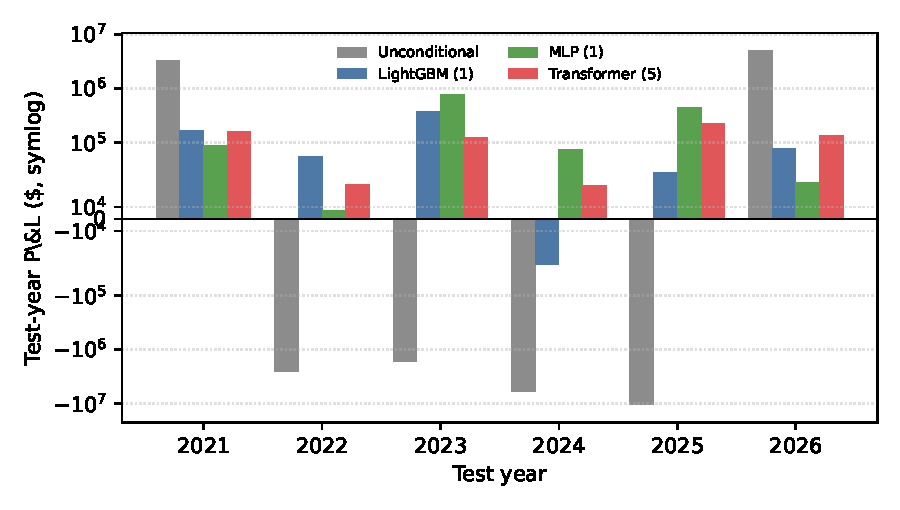
\includegraphics[width=0.66\linewidth]{figures/annual_pnl_bar_chart.pdf}
\caption{Test-year P\&L by model and year, 2021--2026 (Table~\ref{tab:folds}), for the unconditional baseline and the three learned models at a matched single seed (42), each trading only when calibrated probability $\ge 0.5$. Every bar uses the same fixed \$1{,}000 normalized exposure, no reinvestment (Section~\ref{sec:labels}). Symmetric-log $y$-axis, one shared scale (not dual-axis): unconditional's swings are roughly one to two orders of magnitude larger than any learned model's in most years.}
\label{fig:annualpnl}
\end{figure}

\subsection{Training-Window-Length Sensitivity}
\label{sec:window}
An expanding training window (every year from 2014 to the validation year) versus the fixed three-year default, for the primary plain-attention transformer, favors the fixed default on Sharpe in five of six test years; the expanding window earns more raw dollars (\$734.9K versus \$686.2K, from higher 2025--2026 volume at lower average quality) but is the only setting with a negative Sharpe year (2024: $-0.13$ versus 1.59). We keep the fixed three-year window.

\subsection{Additional Robustness Checks}
\label{sec:addl-robustness}
The year-level paired bootstrap treats each test year as one observation. A moving block bootstrap~\cite{kunsch1989} (21-day blocks, 20{,}000 resamples, resampled against unconditional on the real trading calendar) finds the Sharpe gain over unconditional significant for MLP and both transformer variants but \emph{not} LightGBM ($[-0.03, 4.13]$); total-P\&L differences are significant for none, matching the right-skewed swings in Figure~\ref{fig:annualpnl}. Because we evaluated $\sim$21 configurations on the same window (the rows of Table~\ref{tab:consolidated} plus the MV-ALiBi, no-history, expanding-window, probability-floor, and selection-rule variants), a Deflated Sharpe Ratio~\cite{bailey2014deflated} correcting the best observed Sharpe for this multiple testing and for skew/kurtosis gives even the strongest result (MLP, Sharpe 2.60) only $\text{DSR}\approx0.85$ -- short of $0.95$, a further reason not to crown any single configuration.

For market-neutrality we regress each \emph{trade's} return on the underlying's return over that trade's own holding window, rather than a same-day daily-P\&L-on-SPY regression with little power when P\&L books only at exit. All three models show a small but significant \emph{positive} underlying exposure (MLP $\beta{=}7.2$, $t{=}11.5$; transformer $\beta{=}0.9$, $t{=}3.5$; LightGBM $\beta{=}0.7$, $t{=}2.9$) explaining almost no variance ($R^2<0.006$) -- a genuine but economically small directional tilt, largest for the MLP (whose profits are also the most right-skewed), so the strategies are long-biased rather than strictly market-neutral. An average-IV proxy (we did not merge external VIX data from CBOE/FRED) is separately small-but-significant for both transformer variants ($r\approx0.10$, $p<0.005$), not LightGBM or MLP. Entry net delta is predominantly short (75--82\% of trades), a structural consequence of shorting the shorter-dated leg.

Widening execution slippage to 1.5$\times$ the quoted spread at entry leaves every model's positive-year count and ranking unchanged, though Sharpe falls 7--37\% (least sensitive: transformer variants; most: LightGBM). Trades whose short-leg expiration falls on/after the next ex-dividend date carry early-assignment risk the expiration-payoff labels do not price: 16--22\% are exposed, and LightGBM's exposed subset is a net loss ($-\$33$K) while the transformer's has a \emph{higher} win rate than its unexposed one -- a divergence reported without a causal explanation. Finally, because 2026 is a $\sim$107-day partial year (Table~\ref{tab:folds}), we re-ran all metrics on 2021--2025 only: the ranking holds and every learned model stays positive in all five years (MLP single-seed \$1.38M/2.59; five-seed transformer \$532K/1.92), so no conclusion rests on the partial year.

\begin{table}[t]
\footnotesize
\begin{tabular}{lrrr}
\toprule
Model & PR-AUC & Brier & ECE \\
\midrule
LightGBM & 0.492 & 0.086 & 0.049 \\
MLP & 0.406 & 0.096 & 0.036 \\
Transformer (plain, 5-seed) & 0.458 & 0.083 & 0.024 \\
Transformer (ALiBi, 5-seed) & 0.460 & 0.083 & 0.028 \\
No-history ablation, 5-seed (\S\ref{sec:nohistory}) & 0.451 & 0.089 & 0.046 \\
\bottomrule
\end{tabular}
\caption{Precision-recall AUC (average precision), Brier score, and expected calibration error (10 equal-width bins) on the 2021--2026 test-fold population, where the pooled realized base rate is $\approx$13.8\%, identical across models by construction (Section~\ref{sec:lgbm-scope}) -- far below the 25.33\%/23.67\% T1/K2 base rate for the full 2014--2026 sample, reflecting the underlying-price regime shift noted in Section~\ref{sec:limitations}. ROC-AUC is invariant to base rate; we report PR-AUC because it is more sensitive to ranking within the rare positive class, and report ROC-AUC where competition is more balanced (the capital-scaled subset, Section~\ref{sec:capitalscaled}).}
\label{tab:calibration}
\end{table}

Table~\ref{tab:calibration} shows LightGBM has the best discrimination (PR-AUC 0.492) despite lower total P\&L than MLP or the transformer, while the plain-attention transformer has the best calibration (lowest Brier and ECE); no single model dominates every metric, consistent with the finding that P\&L ranking and classification-metric ranking do not always agree. The five-seed no-history ablation's PR-AUC (0.451) is below both transformer variants' -- a second, seed-count-matched line of evidence that historical attention improves discrimination, consistent with the modest matched-seed trading gap in Section~\ref{sec:nohistory}.

\subsection{Capital-Scaled Portfolio Backtest}
\label{sec:capitalscaled}
The \$1,000-per-trade convention used everywhere above isolates selection quality but assumes unlimited capital. We separately simulated realistic position sizing: \$1M starting capital, at most 1\% of available cash committed to new positions each day, equal weighting within a day, no leverage, full P\&L booked at exit, following the position-sizing convention of the companion SPX study~\cite{glasserman2025tp2}. This changes which model looks best (Table~\ref{tab:capitalscaled}): LightGBM and the MLP remain strongly profitable, while both transformer variants, though still ahead of the unconditional baseline, fall far behind on every risk-adjusted metric.

\begin{table}[t]
\centering
\footnotesize
\begin{tabular}{lrrrr}
\toprule
Model & CAGR & Sharpe & Max DD & Calmar \\
\midrule
Unconditional & $-11.7\%$ & $-0.67$ & $-70.5\%$ & $-0.17$ \\
LightGBM & 14.6\% & 1.09 & $-6.3\%$ & 2.31 \\
MLP & 17.2\% & 1.03 & $-5.2\%$ & 3.32 \\
Transformer (plain) & 0.6\% & 0.32 & $-3.7\%$ & 0.18 \\
Transformer (ALiBi) & 0.9\% & 0.51 & $-2.5\%$ & 0.37 \\
\bottomrule
\end{tabular}
\caption{Capital-scaled backtest, 2021--2026, \$1M starting capital and a 1\%-of-cash daily position cap (Section~\ref{sec:capitalscaled}). CAGR and drawdown do not depend on the flat \$1,000-per-trade convention used in Table~\ref{tab:consolidated}.}
\label{tab:capitalscaled}
\end{table}

The cause is an asymmetric payoff shape, not weaker ranking: on each model's lowest-competition (``quiet'') days, where per-trade capital is largest, the transformer wins \emph{more} often than LightGBM/MLP (69.9\% vs.\ 59.8\%/54.9\%) with the best discrimination (AUC 0.906), but its wins are small and losses large (payoff ratio 0.36 versus 4.09/3.54). Its best trades land on its smallest-allocation days, so its flat-notional Sharpe overstates what it captures under a capital constraint -- a limitation of deployability at our sizing convention, not of its selection signal.

\section{Discussion}
\label{sec:discussion}

\subsection{Conditional Selection and the Ensembling Confound}
\label{sec:ensembling-discussion}
The result is conditional selection, not detection: every learned model, including the plain MLP, converts an unconditional loss into a substantial out-of-sample return on the shared $F^{\ast}$ features. Our central comparative finding is a caution, not a claim of superiority. Rankings turn on how ensembling interacts with the fixed decision rule, not architecture alone: ensembling moves both the model and, through recalibration against $p\ge0.5$, its trade count, so seed-count-mismatched comparisons are uncontrolled. Selectivity curves (Section~\ref{sec:selectivity}) separate this from a pure operating-point effect, the single-model gaps are inconclusive at six test years (power $\approx0.26$), and the pattern recurs three times -- MLP-versus-transformer, plain-versus-MV-ALiBi attention, and the no-history ablation. We read the capital-scaled backtest (Section~\ref{sec:capitalscaled}) as the deployment-relevant primary lens; the within-transformer reversal does not survive realistic sizing, under which LightGBM and the MLP are robustly ahead.

\subsection{Threats to Validity}
\label{sec:limitations}
$F^{\ast}$ contains no scale-invariant, moneyness-style price-ratio feature -- every price-level feature is a raw dollar quantity while the underlying drifts 50--80\% across the sample -- the most likely residual regime sensitivity, unaddressed because $F^{\ast}$ is shared across models. We treat TP2 as an empirical violation signal for SPY American calls, not a replication of a theorem proved for European index options~\cite{glasserman2026tp2theory,cosma2020earlyexercise}; robustness to American exercise and dividends is handled at the data level (conservative bid/ask filtering, cost-aware returns), and 16--22\% of selected trades carry short-leg ex-dividend timing (Section~\ref{sec:addl-robustness}). Unlike the companion SPX study~\cite{glasserman2025tp2} we do not additionally filter against a vertical/calendar-spread no-arbitrage condition (reported there to remove $<2\%$ of violations). All code and processed episode/feature/label datasets will be released on acceptance; the raw SPY quote feed is vendor-licensed, but every derived artifact can be redistributed.

\section{Conclusion}
Our central finding is methodological: trading-model rankings turn on how ensembling interacts with the decision rule -- an effect shown at three levels, confirmed under a paired and a block bootstrap, and, with sign-test power only $\approx0.26$ at six test years, unable to separate the architectures either way. The economic setting is itself substantive: unconditional TP2 trading loses money, yet three independent learned selectors each recover a substantial out-of-sample return under one causal, zero-tuning rule. Robustness checks (Sections~\ref{sec:nohistory}--\ref{sec:capitalscaled}) leave the result standing while disclosing real limits: a small trade-level market tilt, historical attention that helps mainly by mechanism rather than by attending to relevant episodes, a best-case Deflated Sharpe of $\approx0.85$, and erosion of the transformer's edge under realistic sizing. The absence of a scale-invariant price feature is the main open problem for future work.

\bibliographystyle{ACM-Reference-Format}
\begingroup
\footnotesize
\setlength{\itemsep}{0pt}
\setlength{\parskip}{0pt}
\begin{thebibliography}{9}

\bibitem{glasserman2025tp2}
Paul Glasserman, Mike Li, and Dan Pirjol. 2025. Trading TP2 Option Violations. Working paper, Columbia Business School and Stevens Institute of Technology.

\bibitem{press2022alibi}
Ofir Press, Noah A. Smith, and Mike Lewis. 2022. Train Short, Test Long: Attention with Linear Biases Enables Input Length Extrapolation. In \textit{International Conference on Learning Representations (ICLR)}.

\bibitem{glasserman2026tp2theory}
Paul Glasserman and Dan Pirjol. 2026. When Are Option Prices TP2? \textit{Mathematical Finance}. Wiley.

\bibitem{glasserman2023convexity}
Paul Glasserman and Dan Pirjol. 2023. Total Positivity and Relative Convexity of Option Prices. \textit{Frontiers of Mathematical Finance} 2, 1 (2023), 1--32.

\bibitem{ke2017lightgbm}
Guolin Ke, Qi Meng, Thomas Finley, Taifeng Wang, Wei Chen, Weidong Ma, Qiwei Ye, and Tie-Yan Liu. 2017. LightGBM: A Highly Efficient Gradient Boosting Decision Tree. In \textit{Advances in Neural Information Processing Systems (NeurIPS) 30}. 3146--3154.

\bibitem{zadrozny2002transforming}
Bianca Zadrozny and Charles Elkan. 2002. Transforming Classifier Scores into Accurate Multiclass Probability Estimates. In \textit{Proceedings of the 8th ACM SIGKDD International Conference on Knowledge Discovery and Data Mining (KDD)}. 694--699.

\bibitem{cosma2020earlyexercise}
Antonio Cosma, Stefano Galluccio, Paola Pederzoli, and Olivier Scaillet. 2020. Early Exercise Decision in American Options with Dividends, Stochastic Volatility, and Jumps. \textit{Journal of Financial and Quantitative Analysis} 55, 1 (2020), 331--356.

\bibitem{kearns2013mlmicrostructure}
Michael Kearns and Yuriy Nevmyvaka. 2013. Machine Learning for Market Microstructure and High Frequency Trading. In \textit{High-Frequency Trading: New Realities for Traders, Markets and Regulators}. Risk Books.

\bibitem{efron1993bootstrap}
Bradley Efron and Robert J. Tibshirani. 1993. \textit{An Introduction to the Bootstrap}. Chapman \& Hall/CRC, New York.

\bibitem{kunsch1989}
Hans R. K\"unsch. 1989. The Jackknife and the Bootstrap for General Stationary Observations. \textit{Annals of Statistics} 17, 3 (1989), 1217--1241.

\bibitem{bailey2014deflated}
David H. Bailey and Marcos L\'opez de Prado. 2014. The Deflated Sharpe Ratio: Correcting for Selection Bias, Backtest Overfitting, and Non-Normality. \textit{Journal of Portfolio Management} 40, 5 (2014), 94--107.

\bibitem{harvey2016crosssection}
Campbell R. Harvey, Yan Liu, and Heqing Zhu. 2016. $\ldots$ and the Cross-Section of Expected Returns. \textit{Review of Financial Studies} 29, 1 (2016), 5--68.

\bibitem{white2000reality}
Halbert White. 2000. A Reality Check for Data Snooping. \textit{Econometrica} 68, 5 (2000), 1097--1126.

\bibitem{hansen2005spa}
Peter R. Hansen. 2005. A Test for Superior Predictive Ability. \textit{Journal of Business \& Economic Statistics} 23, 4 (2005), 365--380.

\bibitem{bouthillier2021accounting}
Xavier Bouthillier et al. 2021. Accounting for Variance in Machine Learning Benchmarks. In \textit{Proceedings of Machine Learning and Systems (MLSys)} 3.

\bibitem{dodge2019show}
Jesse Dodge, Suchin Gururangan, Dallas Card, Roy Schwartz, and Noah A. Smith. 2019. Show Your Work: Improved Reporting of Experimental Results. In \textit{Proceedings of EMNLP-IJCNLP}. 2185--2194.

\bibitem{melis2018state}
G\'abor Melis, Chris Dyer, and Phil Blunsom. 2018. On the State of the Art of Evaluation in Neural Language Models. In \textit{International Conference on Learning Representations (ICLR)}.

\bibitem{lucic2018gans}
Mario Lucic, Karol Kurach, Marcin Michalski, Sylvain Gelly, and Olivier Bousquet. 2018. Are GANs Created Equal? A Large-Scale Study. In \textit{Advances in Neural Information Processing Systems (NeurIPS) 31}. 698--707.

\bibitem{agarwal2021deep}
Rishabh Agarwal, Max Schwarzer, Pablo Samuel Castro, Aaron Courville, and Marc G. Bellemare. 2021. Deep Reinforcement Learning at the Edge of the Statistical Precipice. In \textit{Advances in Neural Information Processing Systems (NeurIPS) 34}. 29304--29320.

\bibitem{grinsztajn2022why}
L\'eo Grinsztajn, Edouard Oyallon, and Ga\"el Varoquaux. 2022. Why Do Tree-Based Models Still Outperform Deep Learning on Typical Tabular Data? In \textit{Advances in Neural Information Processing Systems (NeurIPS) 35 Datasets and Benchmarks}.

\bibitem{shwartzziv2022tabular}
Ravid Shwartz-Ziv and Amitai Armon. 2022. Tabular Data: Deep Learning Is Not All You Need. \textit{Information Fusion} 81 (2022), 84--90.

\bibitem{gorishniy2021revisiting}
Yury Gorishniy, Ivan Rubachev, Valentin Khrulkov, and Artem Babenko. 2021. Revisiting Deep Learning Models for Tabular Data. In \textit{Advances in Neural Information Processing Systems (NeurIPS) 34}. 18932--18943.

\bibitem{shaw2018self}
Peter Shaw, Jakob Uszkoreit, and Ashish Vaswani. 2018. Self-Attention with Relative Position Representations. In \textit{Proceedings of NAACL-HLT}. 464--468.

\bibitem{raffel2020t5}
Colin Raffel et al. 2020. Exploring the Limits of Transfer Learning with a Unified Text-to-Text Transformer. \textit{Journal of Machine Learning Research} 21, 140 (2020), 1--67.

\bibitem{ying2021graphormer}
Chengxuan Ying et al. 2021. Do Transformers Really Perform Badly for Graph Representation? In \textit{Advances in Neural Information Processing Systems (NeurIPS) 34}. 28877--28888.

\bibitem{li2024fire}
Shanda Li et al. 2024. Functional Interpolation for Relative Positions Improves Long Context Transformers. In \textit{International Conference on Learning Representations (ICLR)}.

\bibitem{bali2023option}
Turan G. Bali, Heiner Beckmeyer, Mathis M\"orke, and Florian Weigert. 2023. Option Return Predictability with Machine Learning and Big Data. \textit{Review of Financial Studies} 36, 9 (2023), 3548--3602.

\end{thebibliography}
\endgroup

\end{document}
